{
{\sffamily Her præsenteres forslag til forbedringer af vores
implementering og analyse. Nogle af forslagene kan dog overlappe.
}

\subsection{Udtrækning af regioner}
\begin{itemize}
     \item \textbf{Bedre udtrækning af regioner}\\
        Det er oplagt at implementere bedre udtrækning af regioner.
     \item \textbf{Automatisk udregning af tærskelværdier}\\
        Med vores nuværende udtrækning af regioner ville en
        autogenerering af optimale tærskelværdier for hvert billede
        være yderst gavnligt for udtrækningen af regioner.
    \item \textbf{Fuld segmentering af billedet}\\
        I stedet for kun at finde regioner i forhold til et snit i
        billedet, kunne man trække alle regioner ud med det samme. Dette
        vil gøre det lettere at vurdere regionerne i billedet, og man
        vil således også let, kunne afgøre om en region ligger i flere snit.
  \item \textbf{Egen, eller bedre, implementering af floodfill}\\
        Den floodfill-metode, som er suppleret af \emph{OpenCV}, giver
        kun areal og afgrænsende rektangel for en farvet region. Vi
        ønsker imidlertid flere informationer om regionen, således at
        det ikke er nødvendigt at approksimere regionen med brug af et
        gitter.
    \item \textbf{Mere sofistikeret valg af tilfældig farve}\\
        Valg af tilfældig farve skal tilpasses således, at vi ikke
        vælger en farve, som ligger indenfor den tilladte afvigelse.
        Vi vil også gerne undgå at vælge en farve, som er i billedet i
        forvejen.
    \item \textbf{Mere målrettet udvælgelse af interessante regioner}\\
        Det kunne være interessant kun at klassificere regioner som
        interessante, hvis de var f.eks. et ansigt eller en person.
    \item \textbf{Mere omfattende undersøgelse til fastsættelse af tærskelværdier}\\
		Et mere repræsentativt udvalg af billeder burde kunne give et
		bedre indblik i hvor præcis, denne udviklede implementering er.
		Samt ville give bedre resultater.
\end{itemize}

\subsection{Vurdering af regioner}
\begin{itemize}
    \item \textbf{Sammensmeltning af naiv og udvidet løsning}\\
        Udvikling af en kombination af den naive og udvidede vurdering
		af regioner, således
        at både regioner, der ligger op ad snittet, og dem, der ligger på
        snittet udvælges. Man kunne således også få gjort selve den naive
        vurdering mere sofistikeret ved også at kigge på regionens
        udstrækning.
    \item \textbf{Pointscore i stedet for binær klassifikation}\\
        Dette vil forkaste den binære klassifikation og i stedet give et
        mere præcist mål for, hvorvidt en region ligger i snittet.  Vi
        har allerede givet et forslag til en sådan metode, hvor man kan
        bruge et topografisk kort til at udregne omkostninger for
        regioner.  Regionen kunne approksimeres ved brug af et gitter
        eller dennes konvekse hylster.
    \item \textbf{Bonus for regioner, som ligger i flere gyldne snit}\\
        Det kunne være interessant at undersøge, om fundne regioner
        kvalificerer sig til at ligge i mere end ét gyldent snit. Med
        den nuværende udtrækning \emph{vil} vi have, at hvis en region
        ligger i to snit, så \emph{vil} denne blive trukket ud to gange.
        Vi vil derfor have brug for metoder til at undersøge, om to
        regioner egentlig er den samme. Dette skal løses med en anden
        metode for udtrækning af regioner. Ved binær klassificering skal
        det overvejes, hvordan sådanne regioner belønnes. Bruges der i
        stedet pointscore, vil regionens værdi afspejle dennes specielle
        placering.
    \item \textbf{Ligger der interessante regioner i ``Eye of God''?}\\
        Nogle mener, at punktet vist i figur \ref{eye_of_god} er
        specielt interessant i forbindelse med det gyldne snit. Det
        kunne derfor være spændende at undersøge, om der er en tendens
        til at placere interessante regioner omkring dette punkt.
        Ligeledes kunne man undersøge, om
        interessante regioner følger bestemte linjer i billedet, f.eks,
        diagonalerne indtegnet i figur \ref{eye_of_god} eller den gyldne
        spiral.
    \item \textbf{Er en fundet region konstrueret efter det gyldne snit?}\\
        Det kunne være interessant at undersøge de fundne regioner
        nærmere, for at afgøre, om disse i sig selv er opbygget efter
        det gyldne snit, ligesom vist i utallige malerier af Mona Lisa i
        figur \ref{monalisa_fake}.
\end{itemize}


\subsection{Generelle forbedringer}
\begin{itemize}
    \item \textbf{Mere avanceret database}\\
        En mere avanceret database ville være at foretrække. Der har
        været problemer med SQLite, som låser dele af databasen når man
        arbejder på den. Ligeledes er det værd at overveje en mere
        sofistikeret pakke til databasekommunikation i Python. Det er
        oplagt at bruge \emph{SQLAlchemy}\cite{SQLAlchemy}.
    \item \textbf{Køre analyse på et andet datasæt, som har større diversitet}\\
        Det kunne være interessant, at sammenligne resultater fra en
        analyse på et andet datasæt. Dette ville give os en indikation
		på, om vores resultater fra det oprindelige datasæt kan bruges.
        Ydermere ville det være interessant, at sammensætte et datasæt
        af malerier, hvor det er et faktum, at de er opbygget efter det
        gyldne snit, med det formål at afprøve metoderne på dette.
    \item \textbf{Implementere programmet i et andet sprog}\\
        For en hurtigere analyse af malerier kunne programmet
        implementeres i $\textrm{C}^{++}$, som \emph{OpenCV} er
        implementeret i. Programmet kunne med fordel parallelliseres.
    \item \textbf{Distribueret analyse af billeder}\\
        Med en distribueret løsning til analyse af malerier, ville man,
        ved at lade flere maskiner deles om arbejdet, kunne få
        hastigheden på analysen op.
    \item \textbf{Webservice}\\
        Webservice, hvor klienter kan sende resultater fra kørsel på
        egen maskine, kan udvides til at man selv organiserer billeders
        metadata, således at man ikke er afhængig af et eksternt
        kilde til billeder.
\end{itemize}

\begin{figure}[!h]
    \centering
    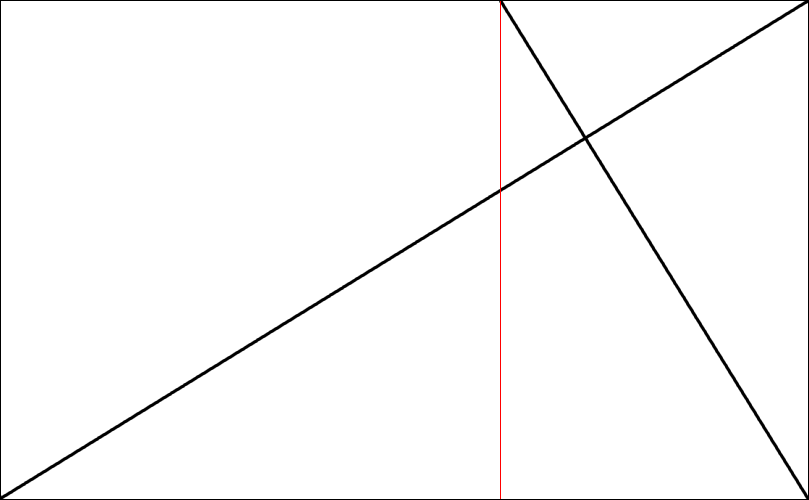
\includegraphics[angle=0,width=0.4\textwidth]{afsnit/fremtidigt_arbejde/billeder/eye_of_god}
    \caption[]{Punktet, hvor de to sorte linjer krydser, kaldes ``The Eye
    of God'' og er her vist i et gyldent rektangel.}
    \label{eye_of_god}
\end{figure}

\begin{figure}[!h]
    \centering
    \subfloat[Leonardo da Vinci: \emph{Mona Lisa} -- 1503--1505/1507 --
    Original]{
    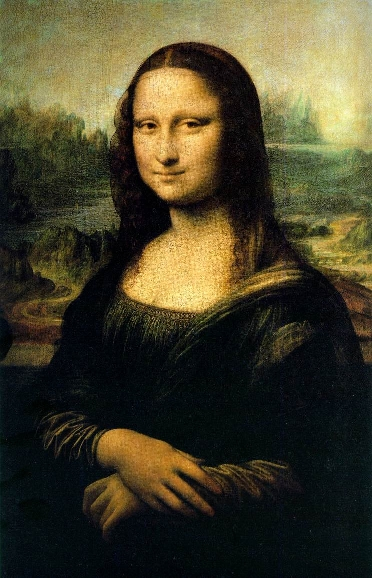
\includegraphics[angle=0,width=0.4\textwidth]{afsnit/fremtidigt_arbejde/billeder/Mona_Lisa.jpeg}
    }
    \subfloat[Arbitrære gyldne rektangler]{
    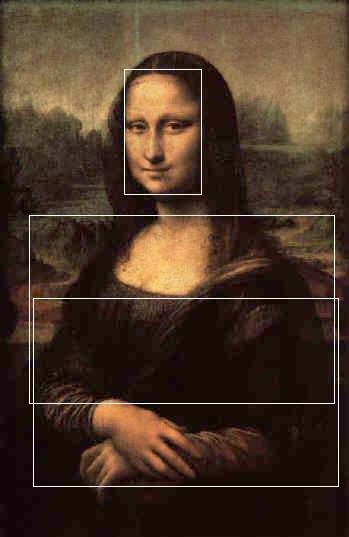
\includegraphics[angle=0,width=0.4\textwidth]{afsnit/fremtidigt_arbejde/billeder/monalisa_fake.jpg}
    }
    \caption[]{Eksempel på regioner, som skulle være
    konstrueret efter det gyldne snit i billedet.}
    \label{monalisa_fake}
\end{figure}


\subsection{Andre forslag inden for området}
\begin{itemize}
    \item \textbf{Bruge teknikker fra HCI til at finde interessante regioner}\\
        Man kunne gøre brug af \emph{eye tracking} til at finde ud af,
        hvor menneskers øjne fokuserer i malerier. En stor undersøgelse
        kunne da give en indikation af, om der findes nogle objekter
        eller steder i malerier, som øjnene automatisk drages mod.
\end{itemize}

}

% vim: set tw=72 spell spelllang=da:
